\chapter{Preliminaries}
\label{chap:prelim}
In the last few years, there has been a rapid development in the field of deep learning application to computer vision and object detection. With each model being an iterative improvement on its predecessors, we review a broad spectrum of neural networks to properly understand the structure and the reasoning behind current state-of-the-art models. This amount of information compels us to leave an explanation of the inner workings of neural networks out of the scope of this thesis. We, therefore, expect prior knowledge from the reader in the area of deep learning, namely in understanding standard modules such as fully connected, convolutional and pooling layers, activation functions, soft-max classifier, batch normalization and principle behind backpropagation and loss functions. All required knowledge can be obtained from the book by \citet{bib:dlbook}.

A large part of this thesis is focused on describing and comparing classification and object detection models, in order to do so, this chapter is dedicated to describing used evaluation metrics and notations.

\section{Evaluation metrics}
In order to evaluate and compare multiple approaches, we require clearly defined evaluation metrics. A state-of-the-art model presented without full specification of used evaluation metrics makes comparing multiple results impossible. Thankfully, there are competitions and challenges with precisely defined rules that are often used to make such comparisons. 

The \textit{ImageNet Large Scale Visual Recognition Challenge }(ILSVRC)\footnote{\url{http://www.image-net.org/challenges/LSVRC/}} is most often used to benchmark classification. Object detection is commonly evaluated in two challenges: the \textit{PASCAL Visual Object Classes Challenge}\footnote{\url{http://host.robots.ox.ac.uk/pascal/VOC/}}, and the \textit{COCO Object Detection Task}\footnote{\url{http://cocodataset.org/}}. Each challenge also provides a public dataset, \textit{ImageNet}, \textit{PASCAL VOC}, and \textit{COCO} respectively.

In this section, we define metrics used to evaluate those challenges, but also other, not considered qualities. Most notably, none of the mentioned challenges is evaluated based on the speed of the model. Since our work is focused on real-time video analysis, we are interested in finding a balance between accuracy and the number of images processed per second (fps). One more factor to consider would be the physical size of the model, usually represented by the number of parameters and directly impacting the amount of needed memory.

\subsection{Classification}
The most common and intuitive evaluation metric for classification problems is the ratio of correctly classified samples. This ratio is referred to as a \textit{classification accuracy}. However, a complement to the accuracy, \textit{top-1 error}, is also often used. In ILSVRC,  alongside top-1 error, a \textit{top-5 error} is used as another major criterion. The top-5 error represents the fraction of test samples in which the correct label does not appear in the top 5 predicted results.

\subsection{Object Detection}
Evaluating a localization and classification of multiple objects in an image is a more complex task than classification, mainly because there is no simple one-to-one mapping between ground-truths and predictions. A ground-truth data are a set of \textit{N} boxes with labels, and detector generates a set of \textit{M} boxes with labels and class confidence values.

Because predicted boxes do not perfectly match ground-truths, a matching algorithm is needed to decide whether a prediction is true positive or false positive. Matching is usually done by computing \textit{intersection over union} (IoU) value for each pair of ground-truth and predicted boxes, and then selecting positive detections based on predetermined threshold.
$$\text{IoU} = \frac{\text{Area}(\text{Prediction} \cap \text{Ground truth})}{\text{Area}(\text{Prediction} \cup \text{Ground truth})}$$

With predictions sorted into true positives (TP), false positives (FP) and false negatives (FN) (no predictions matching a ground-truth box) we are able to calculate \textit{precision} and \textit{recall}.
$$\text{Precision} = \frac{\text{TP}}{\text{TP}+\text{FP}}$$
$$\text{Recall} = \frac{\text{TP}}{\text{TP}+\text{FN}}$$

Now we can define the first metrics used for object detection. Note that all following metrics depend on precision and recall, and therefore depend on the IoU threshold.

\subsubsection{Precision-Recall Curve (PRC)}
PRC is a plot showing the relationship between values of precision and recall. It is plotted separately for each class and reveals how a change in confidence influences the precision and recall values. 

Every point on PRC represents a chosen confidence threshold used for determining positive predictions for a given class. The curve does not show this threshold. Instead, it shows precision and recall received by applying this threshold.

An object detector of a particular class can be considered reliable if its precision stays high while recall increases, which means that predictions with lower confidence score can be considered good predictions.

\subsubsection{Average Precision (AP)}
Comparing curves is not an easy task, particularly if they cross each other frequently, as it often happens with PR curves. However, we can use the area under the PR curve as numerical metrics, called \textit{average precision}. It is usually calculated by interpolation, either on all data points or a small number of equally spaced points (earlier versions of PASCAL VOC Challenge use 11).

Interpolation equation for all points:
$$\sum_{r=0}^1 (r_{n+1} - r_n ) p_{interp}(r_{n+1})$$
with
$$p_{interp}(r_{n+1}) = \max_{\Tilde{r} \geq r_{n+1}} p(\Tilde{r})$$
where $p(\Tilde{r})$ is precision at recall $\Tilde{r}$.

\subsubsection{Mean Average Precision (mAP)}
Comparing two models class by class is impractical, especially with the classifiers for hundreds of classes. Therefore, the most often used metrics for object detectors is a \textit{mean average precision}. As the name suggests, it is a mean of AP across all classes.

Most common notation, mAP@[0.5] means mAP with IoU threshold 0.5. The mAP can also be averaged over multiple IoU thresholds, mAP@[.5, .95] denotes the average mAP from IoU 0.5 to 0.95 usually with step 0.05.

\subsection{Inference Time}
Inference time is a significant factor to consider for the model in real-time application use. With the state-of-the-art models, images are often processed under a second, often in a few milliseconds. Such small numbers can be hard to comprehend. Therefore a more intuitive metric is used. That being the number of processed \textit{frames per second} (fps). However, unlike precision metrics, the fps values are heavily dependant on hardware, software framework, batch size and amount of pre- and post-processing included in the measurement. Hence, only the measurements performed in the identical hardware and software environment are suitable for comparison.

\section{Notation and Convention}
\label{sec:notation}
To avoid any confusion, we define the standard notation used throughout this thesis. We tried to follow the general convention, but there can be some variance compared to other works.

\subsubsection*{Data}

To represent the size of the multidimensional data (tensors), we use bracket notation with dimensional sizes separated by $\times $ sign (not to be confused with multiplication).

A two-dimensional matrix represented as \textbf{[a\x b]}, is most often used to represent spatial dimensions of an image or a feature map. 

In three dimensional data, denoted as \textbf{[a\x b\x c]}, the first two numbers represent the spatial dimension and \textit{c} represents the number of channels, e.g., standard RGB image has three channels. For convenience, we may use \textbf{[a\x c]} notation if \textit{a} and \textit{b} are equal, while explicitly stating the fact.

The next dimension used in neural networks is the batch size \textit{n}. We will be adding this dimension as the last one to our notation, \textbf{[a\x b\x c\x n]}.

We will also be using three-dimensional convolutional layers, that produce five-dimensional tensors. However, we will not add this dimension \textit{d} to the end of the list, but instead, keep channels and the batch size at the end: \textbf{[a\x b\x d\x c\x n]}. 

We sorted the values to allow for unambiguous reference of data without listing every dimension, provided the context of two (2d) or three-dimensional (3d) convolution. For example, data passing between two-dimensional convolutional layers is in the form of four-dimensional tensor, but we will often use only spatial dimensions or spatial and channel dimension to describe given tensor.

\subsubsection*{Convolution}
Since convolutional layers are usually chained together, and always work with the data with \textit{channel} dimension, we do not need to state the channel depth of the input data explicitly. We know that if previous convolution outputs data with the size of [a\x b\x c], and we need to apply \textit{k\x k} kernel, the actual size of the kernel is [k\x k\x c]. However, we must expressly state the number of channels outputted from the convolution to receive the full information. This number determines how many times we perform the convolution operation with different kernels. We call this multi-channel output of the convolutional layer a \textit{feature map}.

Unless stated otherwise, the default parameters for the convolutional layer is stride of one, dilation of one, and sufficient padding to allow the spatial dimensions of the output feature map to stay equal to the input ones. The effects of these parameters are illustrated on \cref{fig:convolutions}.

\begin{itemize}
    \item \textbf{Conv. k\x k\x c} : 2d convolutional layer with kernel size \textit{k\x k} and output channel depth of \textit{c}, while using default values for padding, stride and dilation.
    
    \item \textbf{Conv. k\x k\x c /s P:p D:d} : 2d convolutional layer with stride \textit{s}, padding \textit{p} and dilation \textit{d}. 
    
    \item \textbf{Conv3d. k\x k\x k$_3$\x c P:0} : 3d convolutional layer with kernel spatial size \textit{k\x k} and temporal size \textit{k$_3$}, and output channel depth of \textit{c} and zero padding in all dimensions. 
    
    \item \textbf{Conv3d. k\x k\x k$_3$\x c P:p,p,p$_3$} : 3d convolutional layer with spatial dimensions padded by \textit{p} elements and third dimension padded by \textit{p$_3$} elements.
\end{itemize}

\begin{figure}
    \centering
    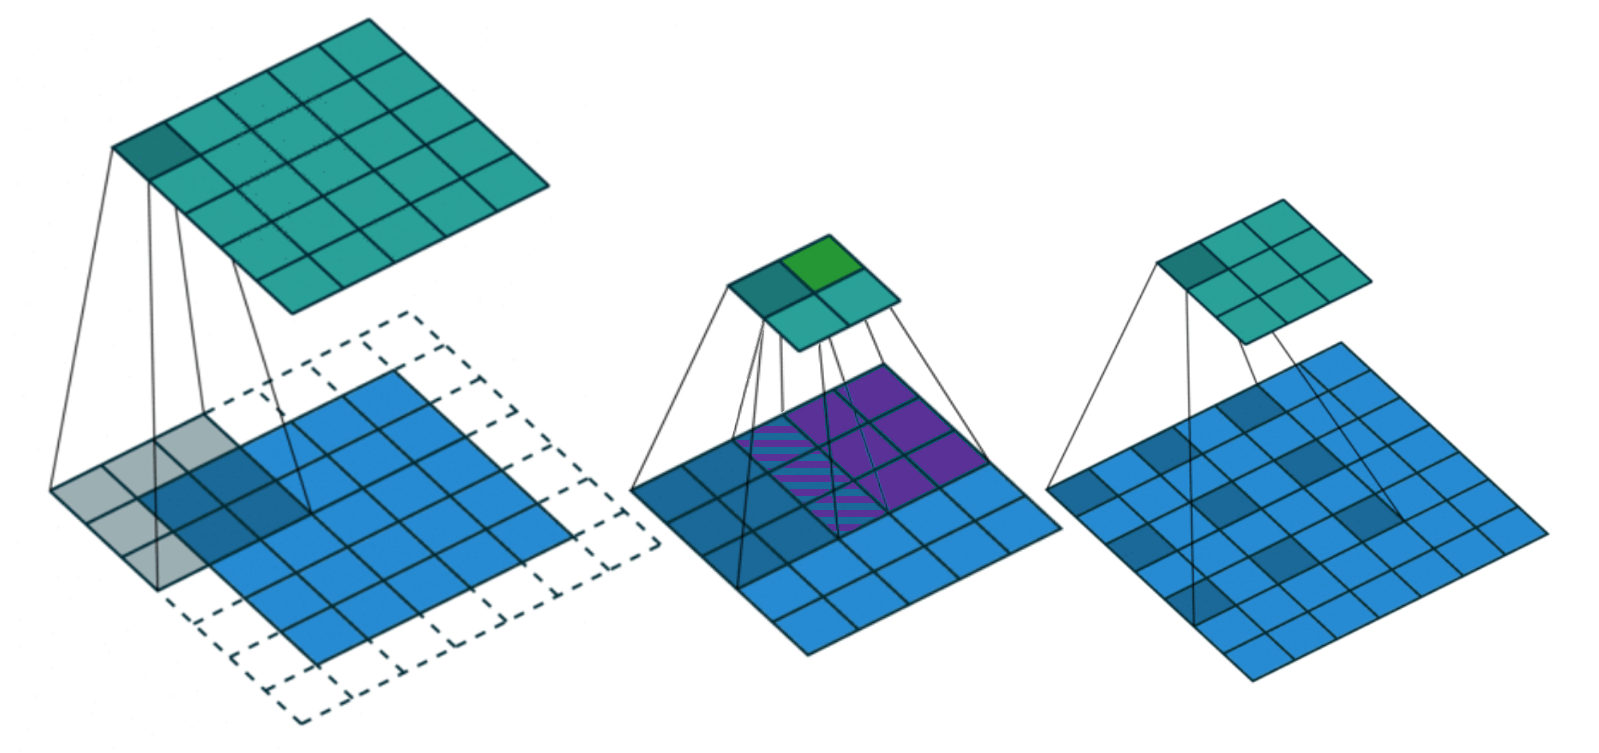
\includegraphics[width=\textwidth]{img/convolutions}
    \caption[Parametrization of convolutional layer]{Effect of padding, stride and dilation on two-dimensional convolutional layer (left to right). Blue maps represent inputs, and cyan maps outputs. Images adopted from \citet{bib:convolution}.}
    \label{fig:convolutions}
\end{figure}

\subsubsection*{Other Layers}
\begin{itemize}
    \item \textbf{Max-pool. k\x k /s P:p} : maximum pooling with kernel size \textit{k\x k}, stride \textit{s} and padding \textit{p}. Default value for stride and padding is 1.
    
    \item \textbf{Fully connected / FC - N} : fully connected layer with \textit{N} neurons
\end{itemize}